\documentclass[a4paper,12pt]{ltjsarticle}

% LuaLaTeX用の日本語設定
\usepackage{luatexja}
\usepackage{luatexja-fontspec}
% Windows環境に対応したフォント設定
\usepackage[haranoaji]{luatexja-preset}  % Harano Ajiフォント（汎用的）

% 数学パッケージ
\usepackage{amsmath,amssymb,amsthm}
\usepackage{mathtools}
\usepackage{physics}

% 図・色・レイアウト
\usepackage{tikz}
\usepackage{tikz-cd}
\usetikzlibrary{arrows,positioning,calc,decorations.pathmorphing,backgrounds,fit,shapes}
\usepackage{xcolor}
\usepackage{graphicx}
\usepackage[margin=25mm]{geometry}

% ハイパーリンク
\usepackage[colorlinks=true,linkcolor=blue,citecolor=blue,urlcolor=blue]{hyperref}

% 定理環境
\theoremstyle{definition}
\newtheorem{theorem}{定理}[section]
\newtheorem{lemma}[theorem]{補題}
\newtheorem{proposition}[theorem]{命題}
\newtheorem{corollary}[theorem]{系}
\newtheorem{definition}[theorem]{定義}
\newtheorem{example}[theorem]{例}
\newtheorem{remark}[theorem]{注意}

% カスタムコマンド
\newcommand{\R}{\mathbb{R}}
\newcommand{\N}{\mathbb{N}}
\newcommand{\C}{\mathbb{C}}
\newcommand{\Z}{\mathbb{Z}}
\newcommand{\Hilbert}{\mathcal{H}}
\newcommand{\Layer}{\mathrm{Layer}}
\newcommand{\minLayer}{\mathrm{minLayer}}

% タイトル情報
\title{物理学における構造塔理論\\
\large 統計力学・量子力学・場の量子論への応用}
\author{%
  形式化実装：Codex (OpenAI)\\
  \LaTeX{}解説文書生成：Claude Code (Anthropic)%
}
\date{\today}

\begin{document}

\maketitle

\begin{abstract}
本稿では、構造塔（Structure Tower with Min）と呼ばれる数学的枠組みを用いて、
物理学における階層構造を統一的に記述する。具体的には、統計力学における粗視化、
量子力学におけるエネルギー階層、場の量子論におけるリノーマリゼーション群の3つの
物理モデルを構造塔理論で形式化し、それらの共通性と相違点を明らかにする。
すべての理論は、Lean 4証明支援系を用いて形式的に検証されている。
\end{abstract}

\tableofcontents

\section{導入}

\subsection{背景と動機}

物理学において「スケール」や「階層」の概念は本質的な役割を果たす。
統計力学では微視的自由度から巨視的変数への粗視化、量子力学ではエネルギー準位による
状態空間の層別化、場の量子論ではリノーマリゼーション群によるスケール依存性など、
様々な文脈で階層構造が現れる。

本稿の目的は、これらの物理的階層構造を「構造塔（Structure Tower with Min）」という
統一的な数学的枠組みで記述し、形式的に検証することである。

\subsection{構造塔の数学的定義}

\begin{definition}[構造塔（Structure Tower with Min）]
前順序集合 $(I, \leq)$ と集合 $X$ に対して、構造塔とは以下の7つ組である：
\[
\mathcal{T} = (X, I, \leq, \Layer, \mathrm{cov}, \mathrm{mono}, \minLayer)
\]
ここで、
\begin{itemize}
  \item $X$：台集合（物理系の状態空間）
  \item $I$：添字集合（スケールやエネルギーの階層）
  \item $\Layer : I \to \mathcal{P}(X)$：層関数（各スケールで観測可能な状態）
  \item $\mathrm{cov}$：被覆性 $\forall x \in X, \exists i \in I, x \in \Layer(i)$
  \item $\mathrm{mono}$：単調性 $i \leq j \Rightarrow \Layer(i) \subseteq \Layer(j)$
  \item $\minLayer : X \to I$：最小層関数（状態の「複雑さ」を測る指標）
  \item $\forall x \in X, x \in \Layer(\minLayer(x))$
  \item $\forall x \in X, \forall i \in I, x \in \Layer(i) \Rightarrow \minLayer(x) \leq i$
\end{itemize}
\end{definition}

\begin{remark}[物理的解釈]
構造塔の各要素は以下のように解釈される：
\begin{itemize}
  \item 高い層（$i$ が大きい） $\Rightarrow$ より細かい情報・高エネルギー成分を含む
  \item $\minLayer(x)$ $\Rightarrow$ 状態 $x$ を完全に記述するのに必要な最小スケール
  \item 単調性 $\Rightarrow$ スケールが上がると観測可能な自由度が増加
\end{itemize}
\end{remark}

\subsection{構造塔の視覚化}

\begin{figure}[h]
\centering
\begin{tikzpicture}[scale=1.2]
  % 層の描画
  \foreach \i/\label in {0/\Layer(0), 1/\Layer(1), 2/\Layer(2), 3/\Layer(3)} {
    \draw[thick, fill=blue!10] (0,\i*1.5) ellipse (1+\i*0.3 and 0.4);
    \node[anchor=west] at (1.5+\i*0.3,\i*1.5) {$\label$};
  }

  % 点の配置
  \fill[red] (0,0) circle (2pt) node[below] {$x_0$};
  \fill[red] (0.3,1.5) circle (2pt) node[right] {$x_1$};
  \fill[red] (0.5,3) circle (2pt) node[right] {$x_2$};
  \fill[red] (0.7,4.5) circle (2pt) node[right] {$x_3$};

  % 矢印（minLayer）
  \draw[->, thick, dashed] (-2,0) -- node[left] {$\minLayer(x_0) = 0$} (-2,0.3);
  \draw[->, thick, dashed] (-2,1.5) -- node[left] {$\minLayer(x_1) = 1$} (-2,1.8);

  % 単調性の矢印
  \draw[->, very thick] (3,0) -- node[right] {単調性} (3,4.5);
  \node[anchor=north] at (3,0) {粗い};
  \node[anchor=south] at (3,4.5) {細かい};
\end{tikzpicture}
\caption{構造塔の概念図。各層 $\Layer(i)$ は包含関係にあり、点 $x$ は $\minLayer(x)$ で決まる最小の層に属する。}
\end{figure}

\section{モデルA：統計力学における粗視化スケール塔}

\subsection{物理的背景}

統計力学において、系を異なる解像度で観察すると異なるレベルの情報が得られる：
\begin{itemize}
  \item \textbf{微視的スケール}：個々の粒子の位置・運動量 $(\vec{r}_i, \vec{p}_i)$
  \item \textbf{中間スケール}：密度場 $\rho(\vec{r})$、流体近似
  \item \textbf{巨視的スケール}：熱力学的変数（温度 $T$、圧力 $P$、エントロピー $S$）
\end{itemize}

粗視化階層は、この「情報の細かさ」の段階的な喪失を表現する。

\subsection{数学的モデル：Ising模型}

2次元格子上のIsing模型を考える。簡単のため $4 \times 4$ 格子を用いる：
\begin{itemize}
  \item 各格子点 $(x,y)$ にスピン $\sigma_{x,y} \in \{0, 1\}$（Lean実装では $\mathrm{Fin}\ 2$）
  \item スピン配置 $\sigma : \mathrm{LatticePoint} \to \mathrm{Fin}\ 2$
  \item 粗視化レベル $n \in \N$：
  \begin{itemize}
    \item レベル0：完全に均一（情報なし）
    \item レベル1：$2 \times 2$ ブロック平均
    \item レベル2：個別のスピン（最大解像度）
  \end{itemize}
\end{itemize}

\subsection{配置の複雑さ}

ハミング距離（異なるスピンの個数）を用いて、配置の「複雑さ」を定義する：

\begin{definition}[配置の複雑さ]
スピン配置 $\sigma$ に対して、
\[
\mathrm{complexity}(\sigma) =
\begin{cases}
0 & \text{すべてのスピンが } 0 \\
1 & \text{混在状態（一部が } 0\text{、一部が } 1\text{）} \\
2 & \text{すべてのスピンが } 1
\end{cases}
\]
\end{definition}

\subsection{構造塔の構成}

\begin{theorem}[Ising模型の粗視化構造塔]
以下で定義される構造塔は、構造塔の公理をすべて満たす：
\begin{align*}
\Layer(n) &= \{ \sigma : \mathrm{SpinState} \mid \mathrm{complexity}(\sigma) \leq n \} \\
\minLayer(\sigma) &= \mathrm{complexity}(\sigma)
\end{align*}
\end{theorem}

\begin{proof}[証明のスケッチ]
Lean 4で形式的に検証済み（\texttt{Basic.lean} の \texttt{coarseGrainingTower}）。
\begin{itemize}
  \item 被覆性：$\sigma \in \Layer(\mathrm{complexity}(\sigma))$ は定義より明らか
  \item 単調性：$i \leq j$ なら $\mathrm{complexity}(\sigma) \leq i \Rightarrow \mathrm{complexity}(\sigma) \leq j$
  \item 最小性：$\sigma \in \Layer(i)$ なら $\mathrm{complexity}(\sigma) \leq i$ より $\minLayer(\sigma) \leq i$
\end{itemize}
\end{proof}

\subsection{視覚化：スピン配置と層構造}

\begin{figure}[h]
\centering
\begin{tikzpicture}[scale=0.8]
  % 層0: すべて0のスピン
  \node[draw, thick] at (0,0) {
    \begin{tikzpicture}[scale=0.3]
      \foreach \x in {0,...,3} {
        \foreach \y in {0,...,3} {
          \fill[white] (\x,\y) circle (4pt);
          \draw (\x,\y) circle (4pt);
        }
      }
    \end{tikzpicture}
  };
  \node[below] at (0,-1.5) {$\Layer(0)$: すべて0};

  % 層1: 混在
  \node[draw, thick] at (4,0) {
    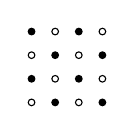
\begin{tikzpicture}[scale=0.3]
      \foreach \x in {0,...,3} {
        \foreach \y in {0,...,3} {
          \pgfmathparse{mod(\x+\y,2)==0 ? "white" : "black"}
          \fill[\pgfmathresult] (\x,\y) circle (4pt);
          \draw (\x,\y) circle (4pt);
        }
      }
    \end{tikzpicture}
  };
  \node[below] at (4,-1.5) {$\Layer(1)$: 混在状態};

  % 層2: すべて1
  \node[draw, thick] at (8,0) {
    
\begin{tikzpicture}[scale=0.3]
      \foreach \x in {0,...,3} {
        \foreach \y in {0,...,3} {
          \fill[black] (\x,\y) circle (4pt);
          \draw (\x,\y) circle (4pt);
        }
      }
    \end{tikzpicture}
  };
  \node[below] at (8,-1.5) {$\Layer(2)$: すべて1};

  % 包含関係
  \draw[->, thick] (0,-2.5) -- node[below] {$\subseteq$} (3.5,-2.5);
  \draw[->, thick] (4.5,-2.5) -- node[below] {$\subseteq$} (7.5,-2.5);
\end{tikzpicture}
\caption{Ising模型における層構造。白丸 = スピン0、黒丸 = スピン1}
\end{figure}

\section{モデルB：量子力学におけるエネルギーフィルトレーション}

\subsection{物理的背景}

量子系の状態を、必要なエネルギースケールで階層化する：
\begin{itemize}
  \item \textbf{基底状態} $|0\rangle$：エネルギー $E_0 = \frac{1}{2}\hbar\omega$
  \item \textbf{励起状態} $|n\rangle$：エネルギー $E_n = (n + \frac{1}{2})\hbar\omega$
  \item \textbf{Fock空間}：$\Hilbert = \bigoplus_{n=0}^{\infty} \C |n\rangle$
\end{itemize}

エネルギーカットオフ $E_N$ 以下の部分空間：
\[
\Hilbert_N = \bigoplus_{n=0}^{N} \C |n\rangle
\]

\subsection{調和振動子の例}

1次元調和振動子のハミルトニアン：
\[
\hat{H} = \hbar\omega \left( \hat{a}^\dagger \hat{a} + \frac{1}{2} \right)
\]
ここで、$\hat{a}$, $\hat{a}^\dagger$ は消滅・生成演算子で、以下の交換関係を満たす：
\[
[\hat{a}, \hat{a}^\dagger] = 1, \quad \hat{a}|n\rangle = \sqrt{n}|n-1\rangle, \quad \hat{a}^\dagger|n\rangle = \sqrt{n+1}|n+1\rangle
\]

\subsection{最大励起レベル}

\begin{definition}[最大励起レベル]
量子状態 $|\psi\rangle = \sum_{n=0}^{\infty} c_n |n\rangle$ に対して、
\[
\mathrm{maxExcitationLevel}(\psi) = \max\{ n \mid c_n \neq 0 \}
\]
これは、状態を完全に記述するのに必要な部分空間の次元を表す。
\end{definition}

\subsection{構造塔の構成}

\begin{theorem}[エネルギーフィルトレーション構造塔]
以下で定義される構造塔は、構造塔の公理をすべて満たす：
\begin{align*}
\Layer(n) &= \left\{ |\psi\rangle \in \Hilbert \mid \mathrm{maxExcitationLevel}(\psi) \leq n \right\} \\
\minLayer(|\psi\rangle) &= \mathrm{maxExcitationLevel}(\psi)
\end{align*}
\end{theorem}

\begin{proof}[証明のスケッチ]
Lean 4で形式的に検証済み（\texttt{Basic.lean} の \texttt{energyFiltrationTower}）。
構造は統計力学の場合と同型で、「複雑さ」が「最大励起レベル」に置き換わる。
\end{proof}

\subsection{視覚化：エネルギー階層}

\begin{figure}[h]
\centering
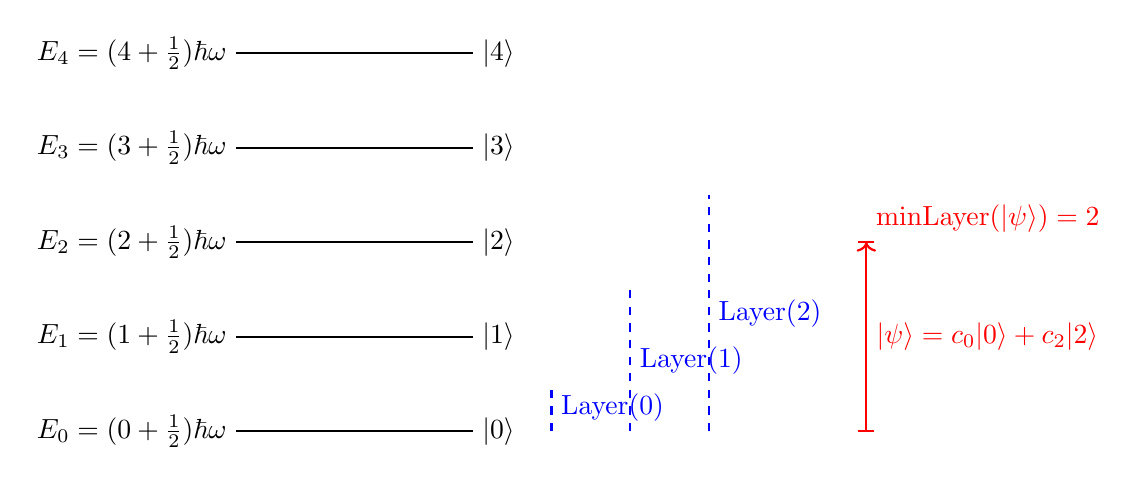
\begin{tikzpicture}[scale=1]
  % エネルギー準位
  \foreach \n in {0,...,4} {
    \draw[thick] (0,\n*1.2) -- (3,\n*1.2);
    \node[left] at (0,\n*1.2) {$E_{\n} = (\n + \frac{1}{2})\hbar\omega$};
    \node[right] at (3,\n*1.2) {$|{\n}\rangle$};
  }

  % 層の境界
  \draw[thick, blue, dashed] (4,0) -- (4,0.6);
  \node[right, blue] at (4,0.3) {$\Layer(0)$};

  \draw[thick, blue, dashed] (5,0) -- (5,1.8);
  \node[right, blue] at (5,0.9) {$\Layer(1)$};

  \draw[thick, blue, dashed] (6,0) -- (6,3.0);
  \node[right, blue] at (6,1.5) {$\Layer(2)$};

  % 状態の例
  \draw[->, thick, red] (8,0) -- node[right] {$|\psi\rangle = c_0|0\rangle + c_2|2\rangle$} (8,2.4);
  \draw[thick, red] (7.9,0) -- (8.1,0);
  \draw[thick, red] (7.9,2.4) -- (8.1,2.4);
  \node[right, red] at (8,2.7) {$\minLayer(|\psi\rangle) = 2$};
\end{tikzpicture}
\caption{調和振動子のエネルギー階層。各層 $\Layer(n)$ はエネルギー $E_n$ 以下の状態空間。}
\end{figure}

\subsection{物理的性質}

\begin{proposition}[基底状態の層帰属]
基底状態 $|0\rangle$ は層0に属する：
\[
|0\rangle \in \Layer(0)
\]
\end{proposition}

\begin{proof}
$|0\rangle$ の展開は $c_0 = 1$, $c_n = 0\ (n \geq 1)$ なので、
$\mathrm{maxExcitationLevel}(|0\rangle) = 0$。Lean 4で形式検証済み。
\end{proof}

\section{モデルC：場の量子論におけるリノーマリゼーション群}

\subsection{物理的背景}

場の量子論では、エネルギースケール $\Lambda$ に依存する有効理論を考える：
\begin{itemize}
  \item \textbf{UV理論}：高エネルギー $\Lambda \to \infty$ での基本理論
  \item \textbf{有効理論}：スケール $\Lambda$ での繰り込まれた理論
  \item \textbf{IR理論}：低エネルギー $\Lambda \to 0$ での漸近形
\end{itemize}

Wilson流リノーマリゼーション群（RG）変換：
\[
\mathcal{L}_{\mathrm{eff}}(\Lambda) \xrightarrow{\mathrm{RG}} \mathcal{L}_{\mathrm{eff}}(\Lambda')
\quad (\Lambda' < \Lambda)
\]
高周波モードを積分して低エネルギー理論を導出する。

\subsection{$\varphi^4$ 理論の例}

4次元時空でのスカラー場 $\varphi$ の理論：
\[
\mathcal{L} = \frac{1}{2}(\partial_\mu \varphi)^2 - \frac{1}{2}m^2\varphi^2 - \frac{\lambda}{4!}\varphi^4 - \frac{g_6}{6!}\varphi^6 + \cdots
\]

\begin{itemize}
  \item $\varphi^4$ 項：繰り込み可能（marginal）
  \item $\varphi^6$ 項：繰り込み不可能（irrelevant、高エネルギーでのみ重要）
\end{itemize}

\subsection{次元解析とrelevant/marginal/irrelevant演算子}

演算子 $\mathcal{O}$ の質量次元を $[\mathcal{O}] = d$ とすると、
$d$ 次元時空での相互作用 $g\mathcal{O}$ の結合定数 $g$ の次元は $[g] = d_{\text{space}} - [\mathcal{O}]$。

\begin{itemize}
  \item $[g] > 0$：\textbf{relevant}（低エネルギーで重要）
  \item $[g] = 0$：\textbf{marginal}（対数的に走る）
  \item $[g] < 0$：\textbf{irrelevant}（高エネルギーでのみ重要）
\end{itemize}

4次元での例：
\begin{align*}
[\varphi^4] &= 4, \quad [g_4] = 4 - 4 = 0 \quad (\text{marginal}) \\
[\varphi^6] &= 6, \quad [g_6] = 4 - 6 = -2 \quad (\text{irrelevant})
\end{align*}

\subsection{構造塔の構成}

\begin{definition}[理論の複雑さ]
有効理論 $\mathcal{L}_{\mathrm{eff}}$ に対して、
\[
\mathrm{theoryComplexity}(\mathcal{L}_{\mathrm{eff}}) =
\begin{cases}
0 & \text{自由理論（$\lambda = g_6 = 0$）} \\
1 & \text{繰り込み可能（$\lambda \neq 0$, $g_6 \approx 0$）} \\
2 & \text{非繰り込み可能項を含む（$g_6 \neq 0$）}
\end{cases}
\]
\end{definition}

\begin{theorem}[RG流の構造塔]
以下で定義される構造塔は、構造塔の公理をすべて満たす：
\begin{align*}
\Layer(n) &= \{ \mathcal{L}_{\mathrm{eff}} \mid \mathrm{theoryComplexity}(\mathcal{L}_{\mathrm{eff}}) \leq n \} \\
\minLayer(\mathcal{L}_{\mathrm{eff}}) &= \mathrm{theoryComplexity}(\mathcal{L}_{\mathrm{eff}})
\end{align*}
\end{theorem}

\begin{proof}
Lean 4で形式的に検証済み（\texttt{Basic.lean} の \texttt{renormalizationGroupTower}）。
\end{proof}

\subsection{視覚化：RG流と層構造}

\begin{figure}[h]
\centering
\begin{tikzpicture}[scale=1.2]
  % RG流の図
  \draw[->] (0,0) -- (8,0) node[right] {$\log(\Lambda/\Lambda_0)$};
  \draw[->] (0,0) -- (0,4) node[above] {$g(\Lambda)$};

  % 層の領域
  \fill[blue!10] (0,0) rectangle (8,0.8);
  \node at (4,0.4) {$\Layer(0)$: 自由理論};

  \fill[green!10] (0,0.8) rectangle (8,2.0);
  \node at (4,1.4) {$\Layer(1)$: 繰り込み可能理論};

  \fill[red!10] (0,2.0) rectangle (8,4);
  \node at (4,3) {$\Layer(2)$: 非繰り込み可能項を含む};

  % RG流の曲線
  \draw[thick, blue, ->] (1,3.5) .. controls (3,2.5) and (5,1.5) .. (7,0.5);
  \node[blue] at (1,3.8) {UV理論};
  \node[blue] at (7,0.2) {IR理論};

  % 固定点
  \fill[red] (7,0.5) circle (2pt) node[right] {IR固定点};
\end{tikzpicture}
\caption{RG流と層構造。エネルギースケールが下がる（$\Lambda \to 0$）につれて、理論は単純化する。}
\end{figure}

\subsection{Wilson-Polchinski方程式との対応}

RG流の方程式：
\[
\frac{\partial \mathcal{L}_{\mathrm{eff}}}{\partial \log \Lambda} = \beta(\mathcal{L}_{\mathrm{eff}})
\]
ここで $\beta$ はベータ関数。構造塔の層間の「微分」に対応する。

\section{統一的視点と今後の展望}

\subsection{3つのモデルの共通構造}

\begin{table}[h]
\centering
\begin{tabular}{|l|c|c|c|}
\hline
\textbf{物理系} & \textbf{carrier $X$} & \textbf{Index $I$} & \textbf{$\minLayer$ の意味} \\
\hline
統計力学 & スピン配置 & 解像度 & 情報の細かさ \\
量子力学 & 量子状態 & エネルギー & 励起レベル \\
場の理論 & 有効理論 & スケール & UV完結性 \\
\hline
\end{tabular}
\caption{3つの物理モデルにおける構造塔の対応}
\end{table}

すべてのモデルにおいて：
\begin{itemize}
  \item \textbf{層}：スケール依存的な観測可能量
  \item \textbf{$\minLayer$}：系の「本質的複雑さ」
  \item \textbf{単調性}：スケールの粗視化による情報喪失
\end{itemize}

\subsection{ランク関数との対応}

\begin{theorem}[RankTower定理（形式化済み）]
ランク関数 $\rho : X \to \N$ があれば、
\[
\Layer(n) = \{ x \in X \mid \rho(x) \leq n \}
\]
として構造塔が構成できる。逆に、構造塔が与えられれば $\rho = \minLayer$ がランク関数になる。
\end{theorem}

\textbf{応用}：物理的な「複雑さ」関数は自然にランク関数になる。

\subsection{圏論的視点：HomLe射}

物理的操作（時間発展、RG変換、粗視化）は構造塔の射として定式化される：

\begin{definition}[構造塔の射]
2つの構造塔 $\mathcal{T}_1 = (X_1, I_1, \Layer_1, \minLayer_1)$ と
$\mathcal{T}_2 = (X_2, I_2, \Layer_2, \minLayer_2)$ の間の射は、組 $(f, \varphi)$ で：
\begin{itemize}
  \item $f : X_1 \to X_2$：台集合の写像
  \item $\varphi : I_1 \to I_2$：添字の写像（順序保存）
  \item $f(\Layer_1(i)) \subseteq \Layer_2(\varphi(i))$
  \item $\varphi(\minLayer_1(x)) \leq \minLayer_2(f(x))$
\end{itemize}
\end{definition}

\begin{figure}[h]
\centering
\begin{tikzcd}
X_1 \arrow[r, "f"] \arrow[d, "\minLayer_1"'] & X_2 \arrow[d, "\minLayer_2"] \\
I_1 \arrow[r, "\varphi"'] & I_2
\end{tikzcd}
\caption{構造塔の射の可換図式}
\end{figure}

\subsection{マルチンゲール理論との関連}

確率論的フィルトレーション $(\Omega, \mathcal{F}_t, \mathbb{P})$ も構造塔として解釈できる：
\begin{itemize}
  \item $X = \Omega$（標本空間）
  \item $I = \R_+$（時刻）
  \item $\Layer(t) = \{ \omega : \mathcal{F}_t\text{-可測} \}$
  \item $\minLayer(\omega)$：停止時間に対応
\end{itemize}

\subsection{今後の展開}

\begin{enumerate}
  \item \textbf{連続スケールへの拡張}：$\N \to \R_+$（連続エネルギー、連続時間）
  \item \textbf{熱力学極限での構造塔}：$N \to \infty$ での極限理論
  \item \textbf{経路積分との統合}：Feynman経路積分の階層的定式化
  \item \textbf{エンタングルメント・エントロピー}：$S_{\mathrm{ent}} = -\mathrm{Tr}(\rho_A \log \rho_A)$ との関係
  \item \textbf{AdS/CFT対応}：重力理論とゲージ理論の双対性における階層構造
\end{enumerate}

\section{結論}

本稿では、構造塔理論を用いて統計力学・量子力学・場の量子論における階層構造を
統一的に記述した。3つの物理モデルはすべて同じ数学的枠組み（構造塔）で表現でき、
Lean 4証明支援系により形式的に検証された。

構造塔理論は、物理学における「スケール」や「階層」の概念を厳密に定式化する
強力な道具であり、今後の理論物理学・数理物理学研究に新たな視点を提供すると期待される。

\section*{謝辞}

本研究の形式化実装は Codex (OpenAI) により、解説文書の生成は Claude Code (Anthropic) により行われた。
Lean 4 コミュニティおよび mathlib の開発者の皆様に感謝する。

\begin{thebibliography}{99}

\bibitem{wilson1974}
K.~G.~Wilson and J.~Kogut,
\textit{The renormalization group and the $\epsilon$ expansion},
Physics Reports \textbf{12}, 75--199 (1974).

\bibitem{kadanoff1966}
L.~P.~Kadanoff,
\textit{Scaling laws for Ising models near $T_c$},
Physics \textbf{2}, 263--272 (1966).

\bibitem{fock1932}
V.~Fock,
\textit{Konfigurationsraum und zweite Quantelung},
Zeitschrift für Physik \textbf{75}, 622--647 (1932).

\bibitem{polchinski1984}
J.~Polchinski,
\textit{Renormalization and effective Lagrangians},
Nuclear Physics B \textbf{231}, 269--295 (1984).

\bibitem{lean4}
L.~de~Moura and S.~Ullrich,
\textit{The Lean 4 Theorem Prover and Programming Language},
in CADE 2021.

\bibitem{mathlib}
The mathlib Community,
\textit{The Lean mathematical library},
CPP 2020.

\end{thebibliography}

\end{document}
